\documentclass{beamer}
\usepackage[utf8]{inputenc}
\usepackage{microtype}
\usepackage{siunitx}
\newcommand{\GR}{{GNU\,Radio}}
\usecolortheme[dark]{solarized}
\title[From my Microphone to the Ether -- an Introduction to SDR]{From my Microphone to the Ether}
\subtitle{An example-based approach to a bit of math}
\author{Marcus Müller}
%\institute{Ettus Research}
\date{Software Defined Radio Academy 2016}
\subject{From my Microphone to the Ether -- an Introduction to SDR}

\usepackage{pgfplots}
\usepgfplotslibrary{fillbetween}
\begin{document}
\frame{\titlepage}


\section{Introduction}

\begin{frame}{Who am I?}
  \begin{itemize}
    \item All-purpose SDR nut
    \item 
\includegraphics[height=2em]{gnuradio_logo} contributor and user
    \item \ldots who was a bit overly present on the \texttt{discuss-gnuradio@gnu.org} mailing list
    \item Got hired by Ettus
  \end{itemize}
  \pause
  \ldots and who is 
\includegraphics[height=2em]{ettus_logo}?
  \begin{itemize}
    \item Producer of the USRP series of SDR frontends
    \item \texttt{gr-uhd} integrates directly in GNU Radio
    \item \texttt{http://www.ettus.com}
    \item mostly directly mixing complex baseband receivers, but many can be used in Low-IF and direct sampling modes!
  \end{itemize}
\end{frame}

\begin{frame}{A short overview}
  \tableofcontents{}
\end{frame}


\section{SDR: A short introduction}

\begin{frame}{What are we after?}

  \only<1>{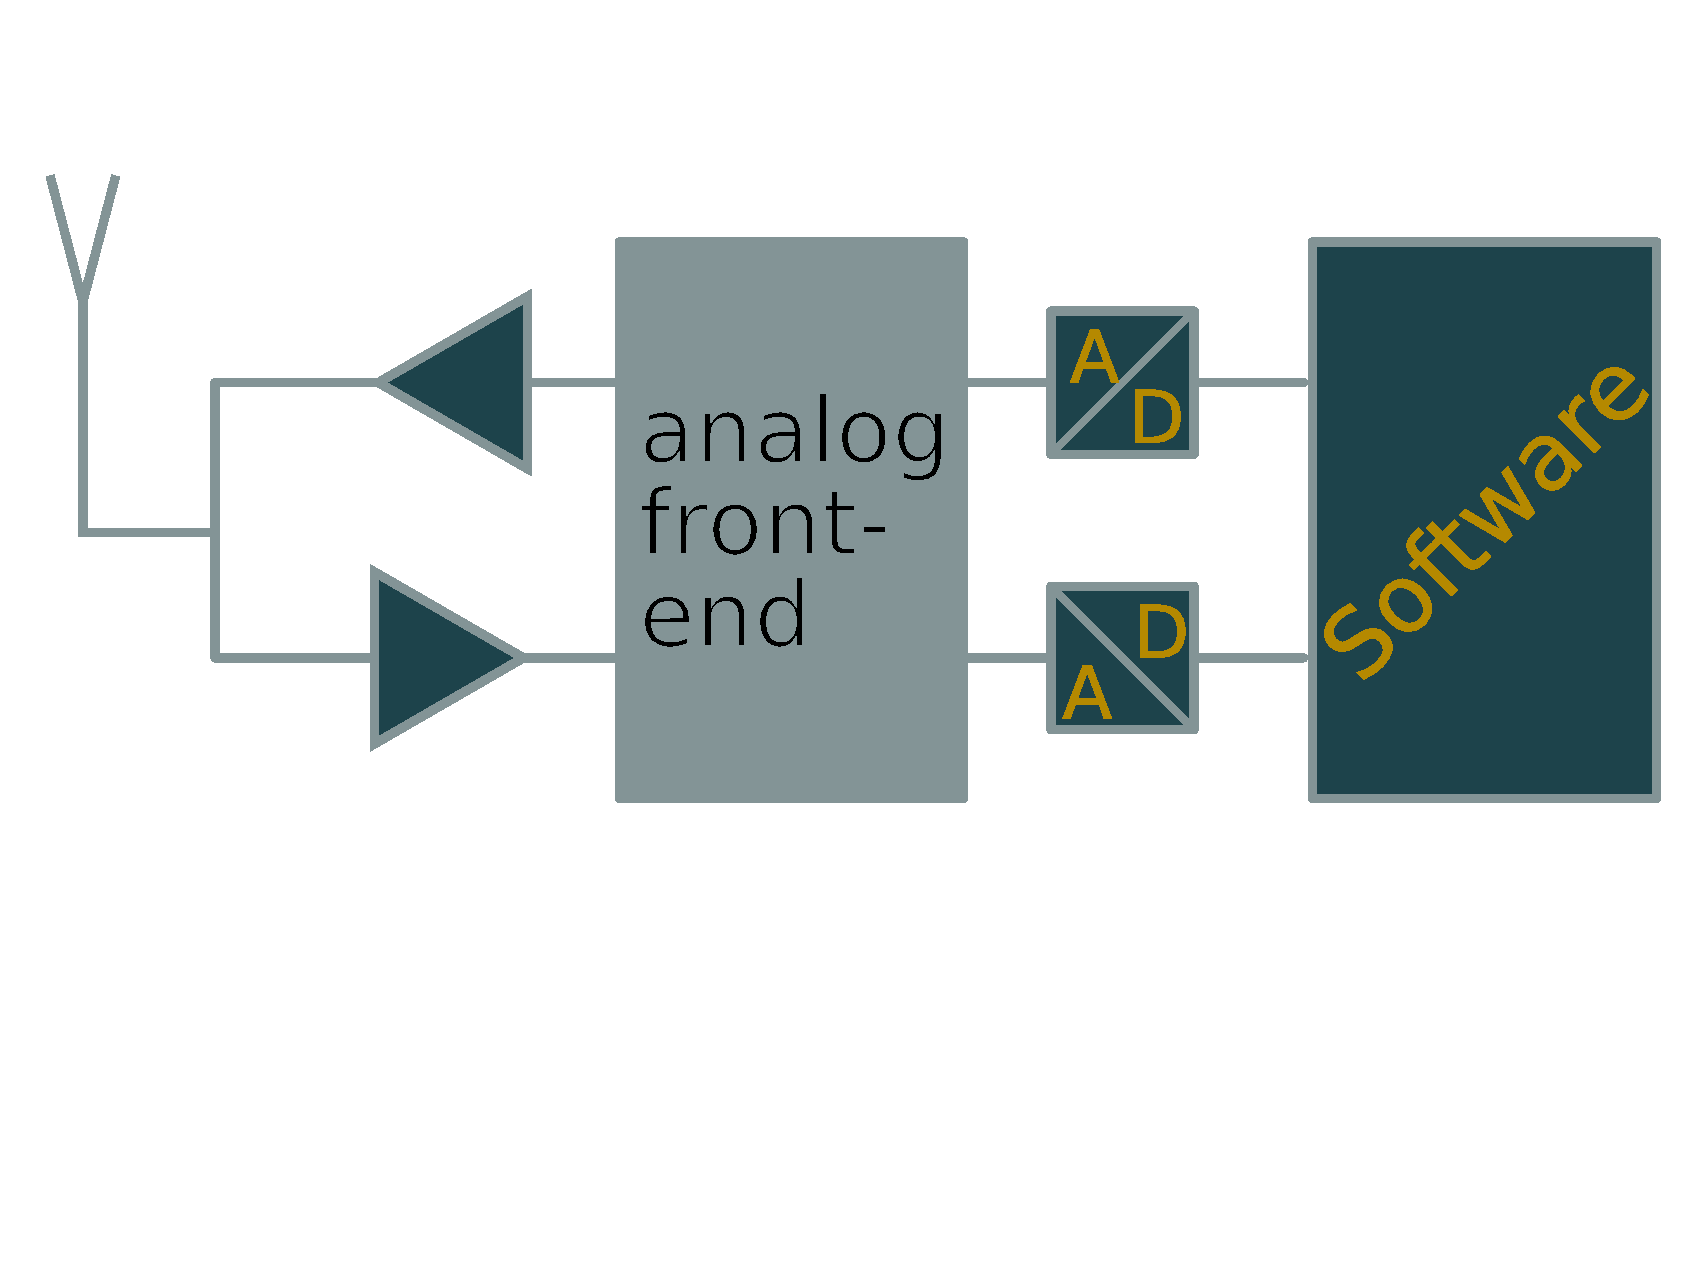
\includegraphics[width=\textwidth]{antsoftware}}

  \only<2>{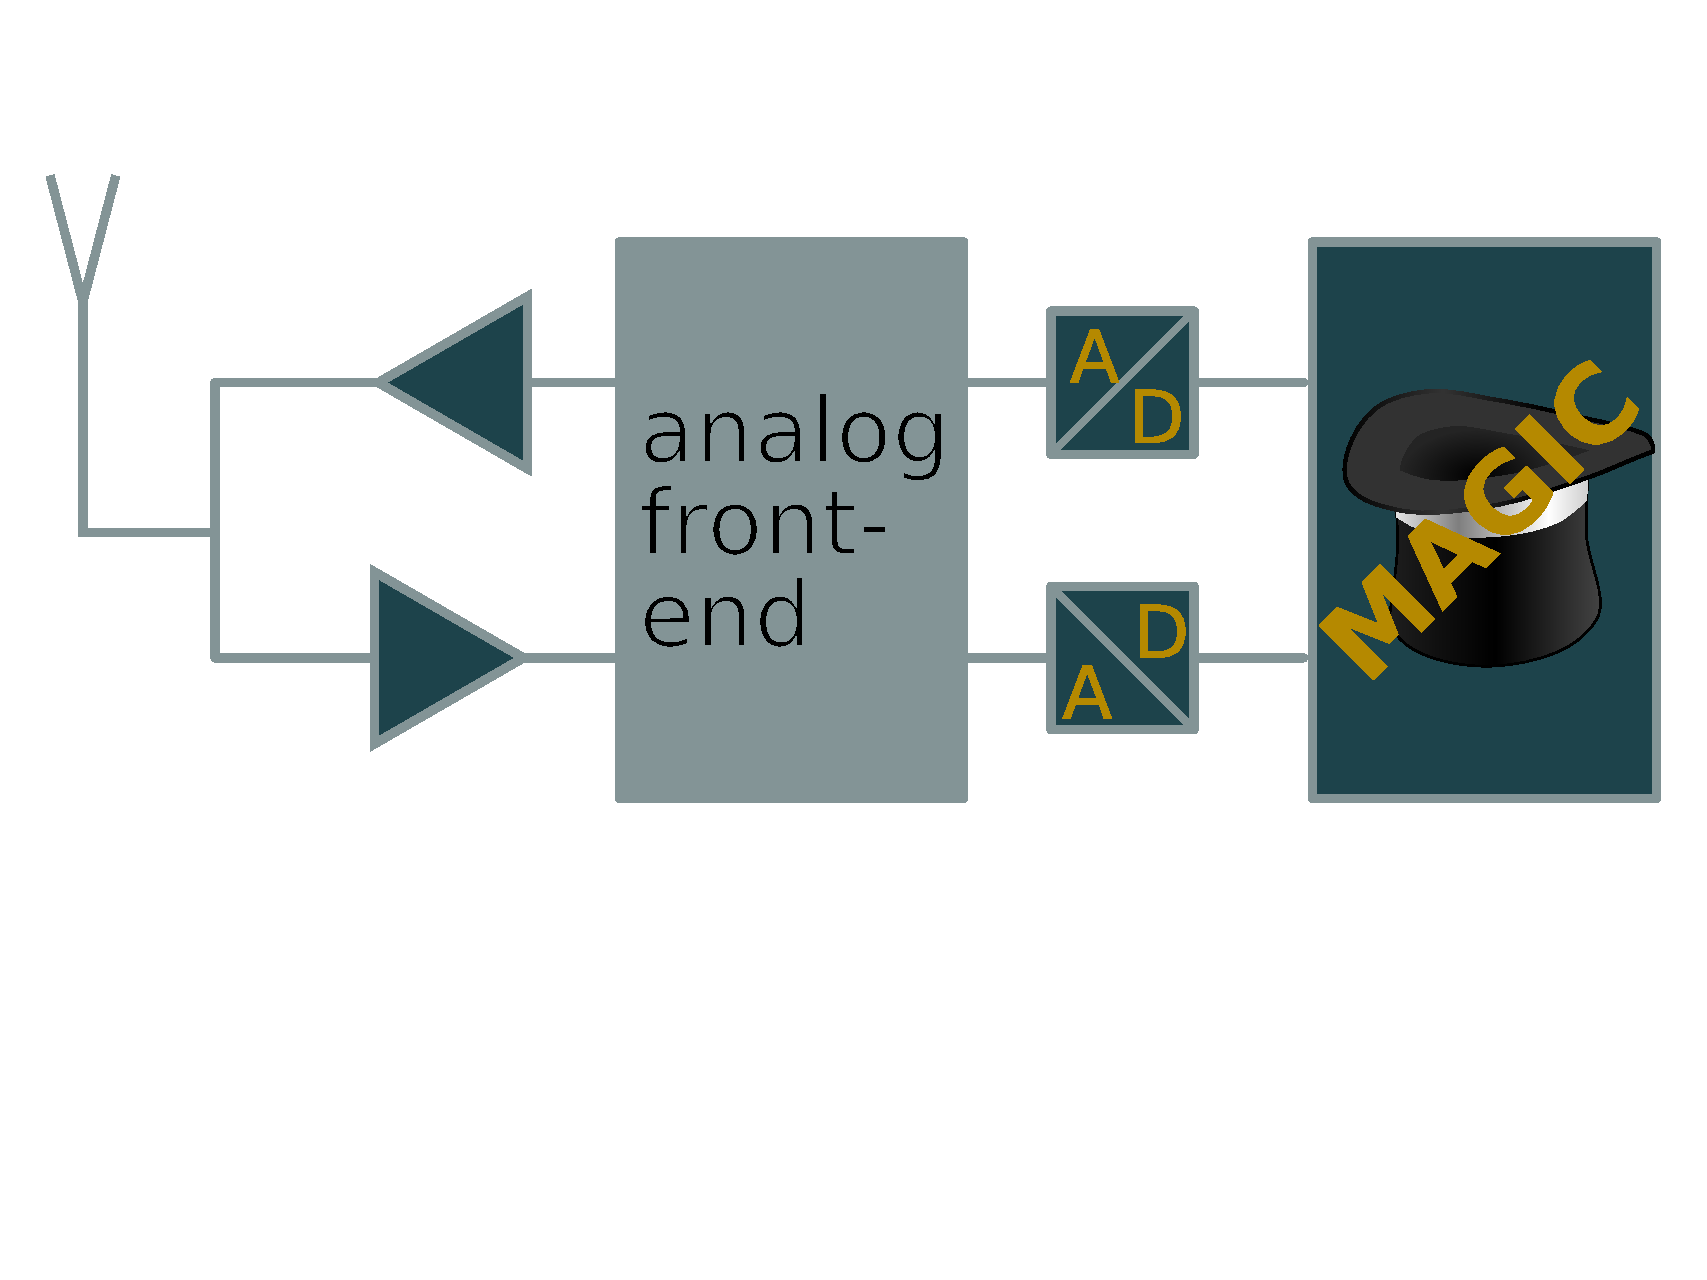
\includegraphics[width=\textwidth]{antsoftwaremagic}}

  \only<3>{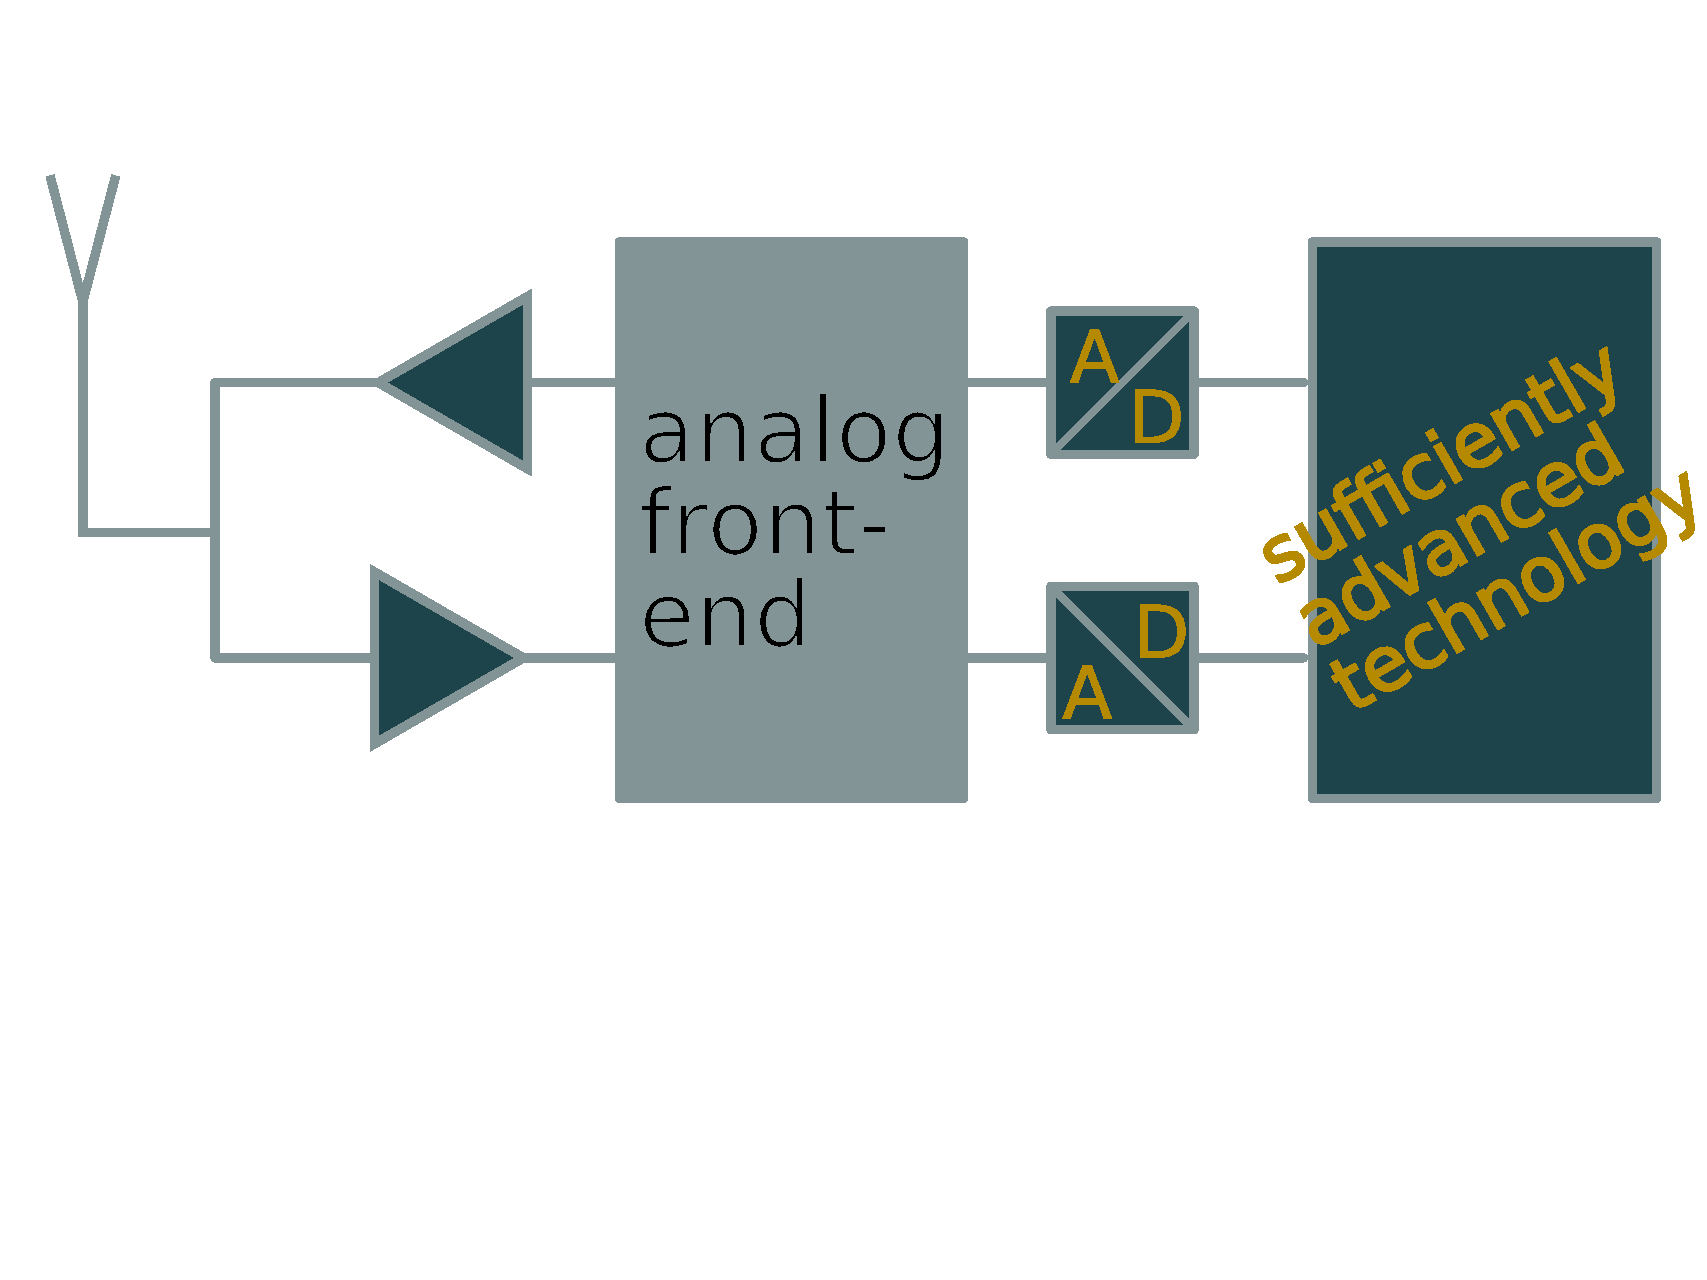
\includegraphics[width=\textwidth]{antsoftwaretechnology}}

  \only<4>{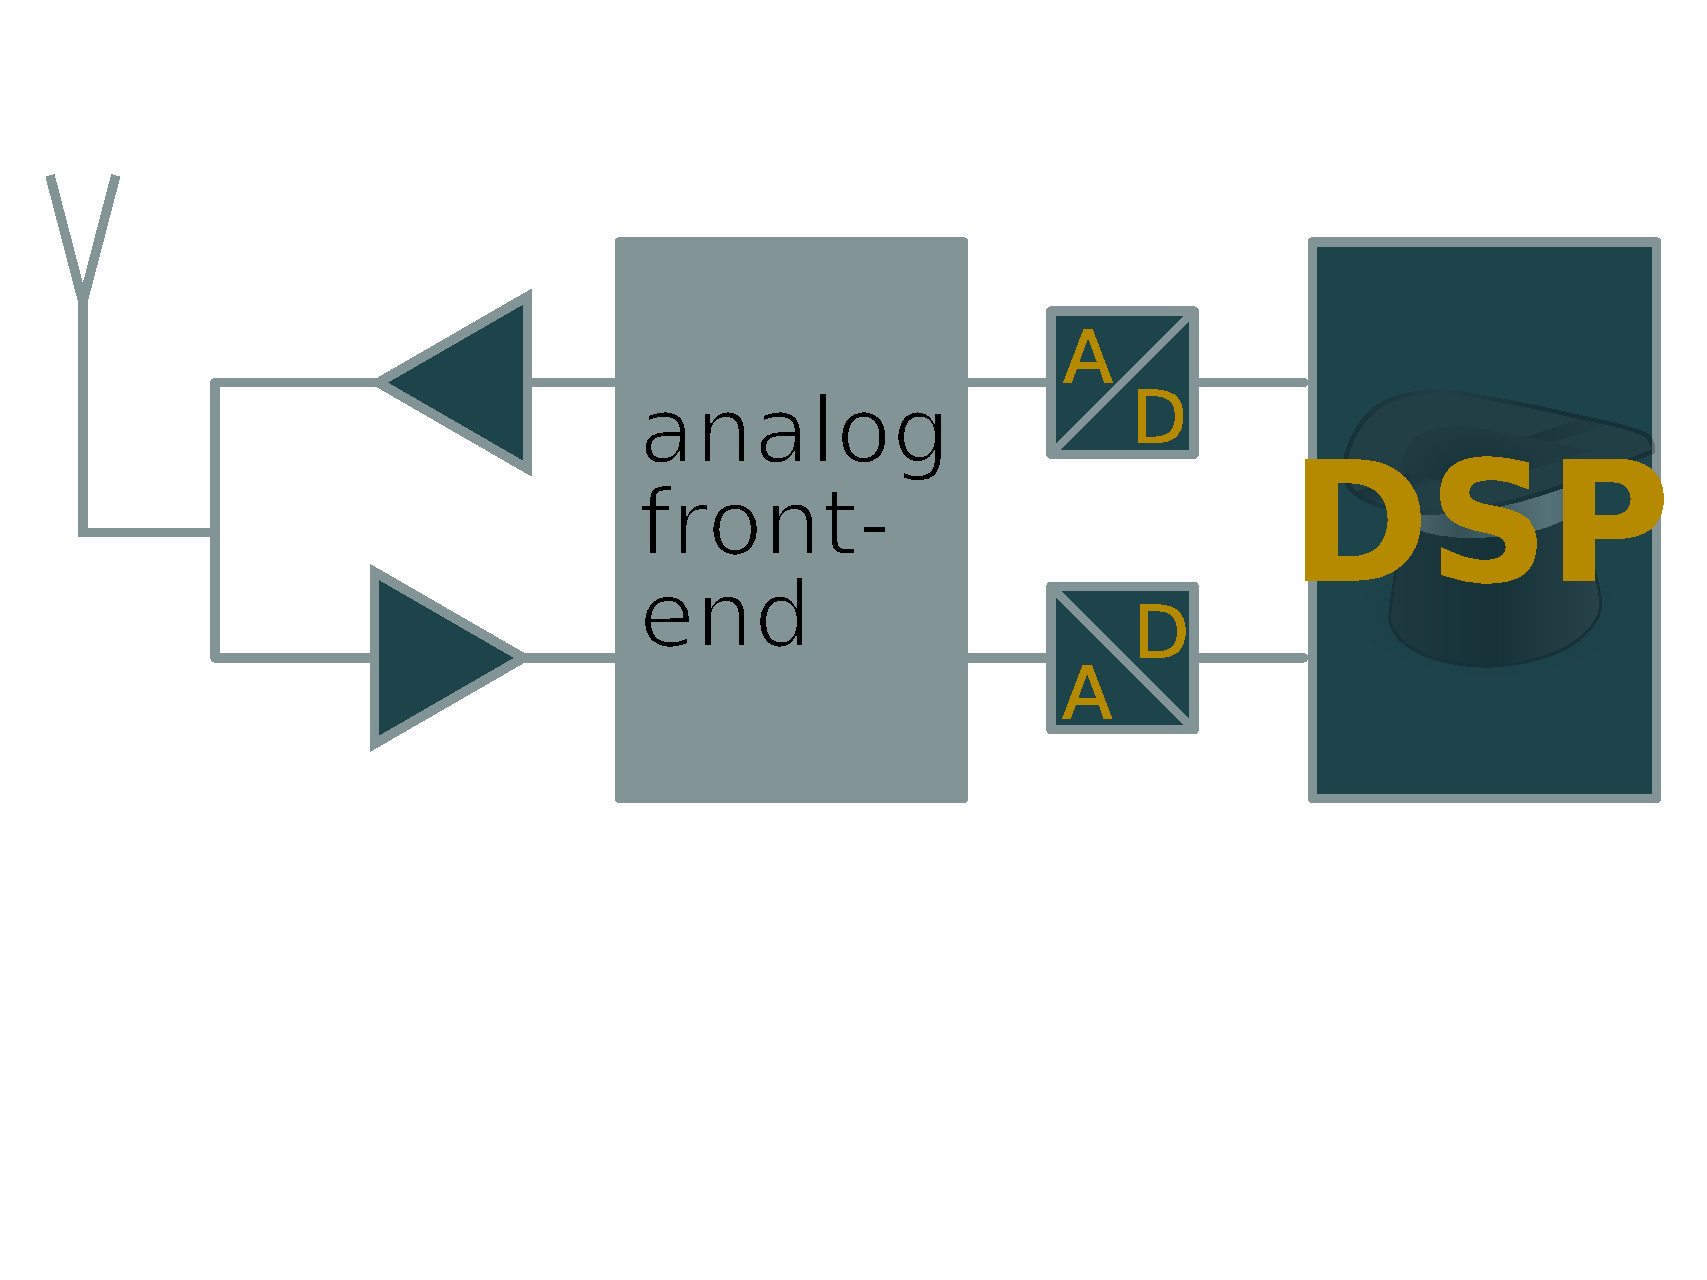
\includegraphics[width=\textwidth]{antsoftwaredsp}}

\end{frame}

\section{Signals and their Spectrum -- math'ing things up}
\begin{frame}{Understanding Signals in the Frequency Domain}
  Fourier states:\\[3em]

  \fbox{\parbox{0.9\textwidth}{Every sufficiently well-behaved\footnote{i.e.
  the signals we care about} signal can be reproduced to an arbitrary amount of
precision by combining harmonic functions}}\\[3em]

Bonus: if they are periodic, it's only a discrete set of harmonics!

\pause{Example: square wave}
\end{frame}

\begin{frame}{Square Wave reconstruction through harmonic functions}
  \input{squarewaves}
\end{frame}

\begin{frame}{Taking a look at the spectrum}


Intuitively, we know that all our sines are just single tones, and will leave a simple line in the spectrum\bigskip

\includegraphics[width=0.45\textwidth]{squarehalf}$\leftrightarrow$\includegraphics[width=0.45\textwidth]{squarespectrumhalf}\bigskip

\pause

\begin{itemize}
  \item The \textbf{Fourier Transform} actually does exactly that: Converting between time domain and frequency domain.
  \item Allows for negative frequencies and complex signals/spectra; a bit much math for 30 minutes
\end{itemize}


\end{frame}

\begin{frame}{Taking a look at the spectrum}

  \only<1>{\includegraphics[width=\textwidth]{square}}

  \only<2>{\includegraphics[width=\textwidth]{squarespectrum}}

\end{frame}

\begin{frame}{Why is this important?}
\only<1>{\begin{itemize}
    \item real-world systems always have a bandwidth-limiting, usually low-pass, behaviour
    \item that leaves us with only a limited amount of spectrum to reproduce the original signal
  \end{itemize}}

      \only<2>{\includegraphics[width=\textwidth]{squarespectrum}}

      \only<3>{\includegraphics[width=\textwidth]{squarespectrum7}}

      \only<4>{\includegraphics[width=\textwidth]{square}}

      \only<5>{\includegraphics[width=\textwidth]{squarerec7}}
\end{frame}

\section{Digital Signal Processing (DSP)}

\begin{frame}{Remember this slide?}

  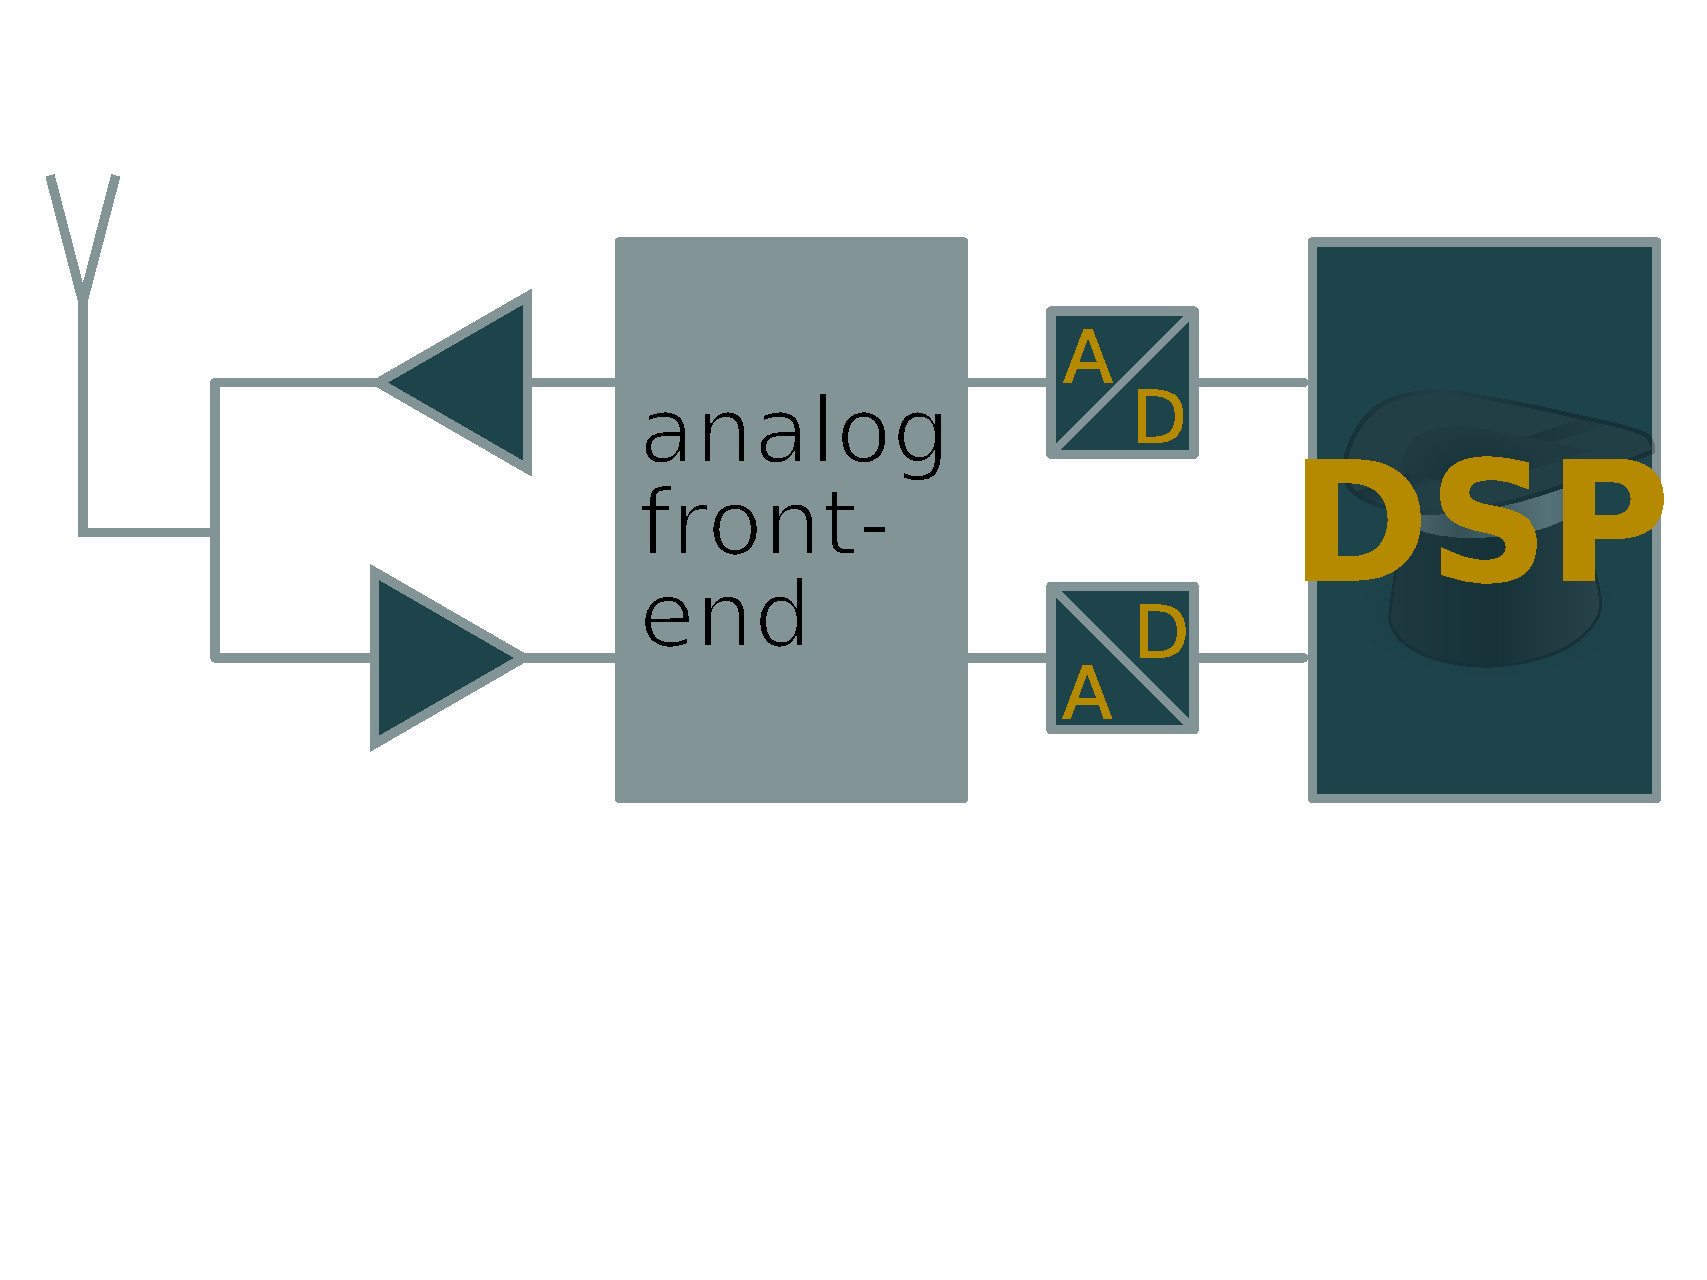
\includegraphics[width=\textwidth]{antsoftwaredsp}

\end{frame}

\begin{frame}{Digital Signal Processing}
\begin{itemize}
  \item works with a digital signal instead of analog things like voltages, currents
  \item typically uses software running on processors or specific hardware to implement all kinds of functionality
    \begin{itemize}
      \item computers are cheap
      \item good filters are expensive
      \item software can much easier be written than implementing e.g. a cell phone in hardware alone
    \end{itemize}
\end{itemize}
\end{frame}

\begin{frame}{What \textit{is} a Digital Signal?}{formally}
  Definition:\\[3em]

  \fbox{\parbox{0.9\textwidth}{A digital signal is a signal that
    \begin{itemize}
    \item only takes discrete values, and
    \item only exists for discrete times.
  \end{itemize}
  }}

\end{frame}

\begin{frame}{What \textit{is} a Digital Signal?}{visually}

  \only<1>{\includegraphics[width=\textwidth]{siganalog}}

  \only<2>{\includegraphics[width=\textwidth]{siganaloggrid}}

  \only<3>{\includegraphics[width=\textwidth]{siganalogdigital}}

  \only<4>{\includegraphics[width=\textwidth]{sigdigital}}

\end{frame}

\begin{frame}{Digital Signals}{are great!}
  \begin{itemize}
  \item can just be represented as series of numbers\\
  \only<1>{\includegraphics[width=\textwidth]{sigdigitalsmall}}
\only<2->{\input{digital}}
\item<3-> which is actually something that computers can work with!
  \end{itemize}
\end{frame}

\begin{frame}{Sampling}{\only<1-2>{Going from Analog to Digital in $N$ discrete Steps}\only<3>{Reconstructing is easy!}\only<4->{Ouch.}}

  \only<1>{\includegraphics[width=\textwidth]{sigcos}}

%  \only<2>{\includegraphics[width=\textwidth]{sigcosperiod}}

  \only<2>{\includegraphics[width=\textwidth]{sigcossampling}}
  
  \only<3>{\includegraphics[width=\textwidth]{sigcossampled}}

  \only<4>{\includegraphics[width=\textwidth]{sigcosundersampled}}

  \only<5>{\includegraphics[width=\textwidth]{sigcosundersampled2}}


\end{frame}


\section{Sampling}

\begin{frame}{Sampling -- Periodicity in Frequency Domain}{}
  \begin{itemize}
    \item<1-> There's \emph{always} ambiguity whether the original periodic signal had frequency $f$ \ldots
    \item<2-> or $f+f_{sample}$ \ldots
    \item<3-> or $f+2f_{sample}$ \ldots
    \item<4-> or, in fact, $f+Nf_{sample}$ for any $N \in \mathbb N$.
  \end{itemize}
\end{frame}
\begin{frame}{Sampling -- Periodicity in Frequency Domain}{}
  when considering a digital signal, its spectrum
  \begin{itemize}
    \item can only meaningfully be defined for a bandwidth of $f_{sample}$,
    \item repeats every $f_{sample}$.
  \end{itemize}

\end{frame}
\begin{frame}{Sampling -- Periodicity in Frequency Domain}{Aliasing}

  Hence: Sampling analog signals demands:\\
  \fbox{\textbf{bandwidth limited sufficiently (filtered)!}}

  \begin{itemize}
    \item frequencies at $f + Nf_{sample}$ ending up at $f$ is called \textbf{aliasing}.
    \item Anti-Aliasing Filter: typically low pass filter
  \end{itemize}

  Works the other way around, too -- \textbf{Images} every $f_{sample}$ when DAC'ing $\rightarrow$ \emph{Reconstruction} filter
\end{frame}
\begin{frame}{Sampling -- Periodicity in Frequency Domain}{Undersampling}
    Alternatively \emph{use} aliasing
      \begin{itemize}
        \item alias a higher range of spectrum into baseband -- \textbf{Undersampling}
        \item works well for relatively low frequencies (filters are easy/affordable/can be build adjustably)
        \item good high-frequency analog filters expensive/hard to make
        \item building a receiver working 0--25 MHz just as well as 5.000--5.025 GHz is physically hard
        \item \ldots and expensive: imagine the loads of filters!
        \item typical frequency agility seen with Ettus USRPs is achieved by first mixing to baseband, and then digitizing
      \end{itemize}
\end{frame}

\begin{frame}{Spectra of Digital Signals}{}

  \begin{itemize}
    \item Example: impossible to tell whether your signal is $\cos(\pi x)$ or $\cos(-\pi x)$:      \includegraphics[width=\textwidth]{sigcossmall}
    \item spectrum of $\cos(\pi x)$ has a isolated  value at both $\pm \frac12$
      \only<1>{\includegraphics[width=\textwidth]{speccossmall}}
    \only<2>{\item and because we've sampled it, it's $f_{sample}$-periodic:
      \includegraphics[width=\textwidth]{speccosperiodsmall}}
  \end{itemize}

\end{frame}

\begin{frame}{Spectra of Digital Signals}{}

  Real Signals: Spectrum is hermitian symmetric

  \begin{itemize}
    \item spectra can be complex (otherwise, we couldn't represent phase of a signal)
    \item $\Re\{S(f)\} = \Re\{S(-f)\}$
    \item $\Im\{S(f)\} = -\Im\{S(-f)\}$
    \item Spectrum Analyzer only shows magnitude of spectrum: Can't tell sign of $\Im\{S\}$
  \end{itemize}

\end{frame}
\begin{frame}{Spectra of Digital Signals}{}

  Real Signals: Spectrum is hermitian symmetric

  \begin{itemize}
    \item Positive half of spectrum fully defines negative half
    \item if symmetric and $f_{sample}$ periodic\ldots
    \item only half of $f_{sample}$ ``usable''
  \end{itemize}

{ $\rightarrow$ \textbf{Sampling Theorem} for real-valued signals}
\end{frame}

\begin{frame}{The Shannon-Nyquist Sampling Theorem}

  \fbox{\parbox{\textwidth}{For real-valued sampling, the observed bandwidth of the analog signal must be limited to less than half the sampling rate.}}\bigskip

\only<1>{
\begin{tikzpicture}
\begin{axis} [
        height=5cm,width=\textwidth,xlabel={$f$},axis lines=middle,
        xmin=-120,xmax=200,ymin=0,ymax=1.8,no markers,
        xtick={80},xticklabels={$\frac{f_{sample}}{2}$},
        ytick={0},yticklabels={},ylabel={$S(f)$}
  ]
    \addplot[thick,fg=solarizedRebase03] coordinates {(-100,0) (-20,1) (0,0)};
    \addplot[thick,fg=solarizedRebase03] coordinates {(0,0) (20,1) (100,0)};
    \addplot[fg=solarizedRebase03,dashed,name path=B] coordinates {(80,0) (80,1.5)};
    \addplot[fg=solarizedRebase03,dashed,name path=C] coordinates {(-80,0) (-80,1.5)};
\end{axis}
\end{tikzpicture}}

\only<2>{
\begin{tikzpicture}
\begin{axis} [
        height=5cm,width=\textwidth,xlabel={$f$},axis lines=middle,
        xmin=-120,xmax=200,ymin=0,ymax=1.8,no markers,
        xtick={80},xticklabels={$\frac{f_{sample}}{2}$},
        ytick={0},yticklabels={},ylabel={$S(f)$}
  ]
    \addplot[thick,fg=solarizedRebase03] coordinates {(-100,0) (-20,1) (0,0)};
    \addplot[thick,fg=solarizedRebase03] coordinates {(0,0) (20,1) (100,0)};
    \addplot[thick,fg=solarizedRebase03,name path=A] coordinates {(60,0) (140,1) (160,0)};
    \addplot[thick,fg=solarizedRebase03,name path=D] coordinates {(-60,0) (-140,1) (-160,0)};
    \addplot[fg=solarizedRebase03,dashed,name path=B] coordinates {(80,0) (80,1.5)};
    \addplot[fg=solarizedRebase03,dashed,name path=C] coordinates {(-80,0) (-80,1.5)};
    \addplot[color=solarizedOrange] fill between[of=A and B,soft clip={domain=60:80}];
    \addplot[color=solarizedOrange] fill between[of=C and D,soft clip={domain=-80:-60}];
\end{axis}
\end{tikzpicture}}

\end{frame}

\begin{frame}{The Shannon-Nyquist Sampling Theorem}

  \fbox{\parbox{\textwidth}{For real-valued sampling, the observed bandwidth of the analog signal must be limited to less than half the sampling rate.}}\bigskip

  Example:
  \begin{itemize}
    \only<1,2>{\item Sound cards sample with 44.1 kHz, 48 kHz or 96 kHz. Human perception reaches roughly from 10 Hz to 16 kHz.}
    \only<2>{\item Understanding voice possible using lower bandwidths -- can find sampling rates of 16 kHz and below in standards.}
    \only<3>{\item superheterodyne receiver:mix 1 MHz of signal from 465.5 -- 4.665 MHz to 69.5 -- 70.5 kHz ($f_c = 70 \text{ MHz}$). 
      \begin{itemize}
        \item when considering 0 Hz -- 70.5 MHz, one would need a sampling rate of at least 141 MHz
        \begin{itemize}
          \item high, but far from impossible (USRPs currently do up to 200 MS/s)
          \item totally unnecessary!
        \end{itemize}
        \item when undersampling, sampling rate of 2 MHz is sufficient
        \begin{itemize}
          \item high requirement for quality of band-pass signal
          \item good SAW filters exist for specific frequencies (reason Superhet is popular, even analog!)
        \end{itemize}
    \end{itemize}}
  \end{itemize}

\end{frame}

\section{Looking at a complete system}
\begin{frame}{Looking at a complete system}

  FM Receiver in GNU Radio \bigskip

  {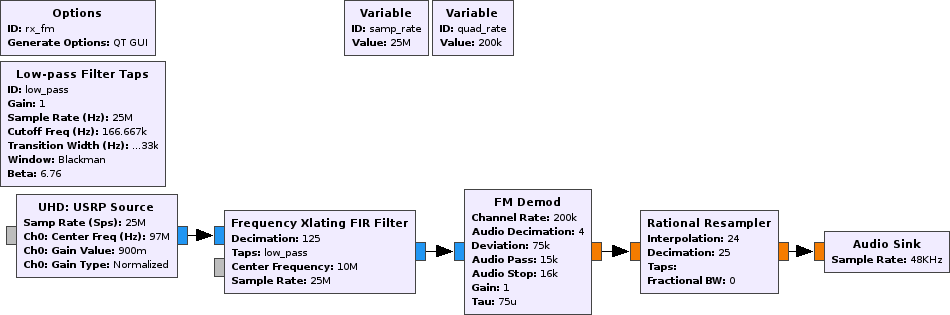
\includegraphics[width=\textwidth]{fg}}



\end{frame}
\begin{frame}{Looking at a complete system}

  FM Receiver in GNU Radio \bigskip


  {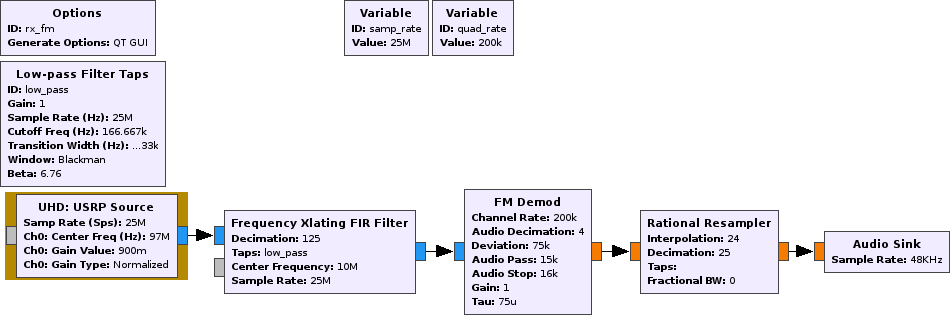
\includegraphics[width=\textwidth]{fg_usrp_source}}

  USRP Source

  \begin{itemize}
    \item interface to the USRP
    \item talks to the driver
    \item configures all analog and DSP aspects of the USRP
    \item receives samples
  \end{itemize}


\end{frame}
\begin{frame}{Looking at a complete system}

  DSP in the USRP \bigskip


  {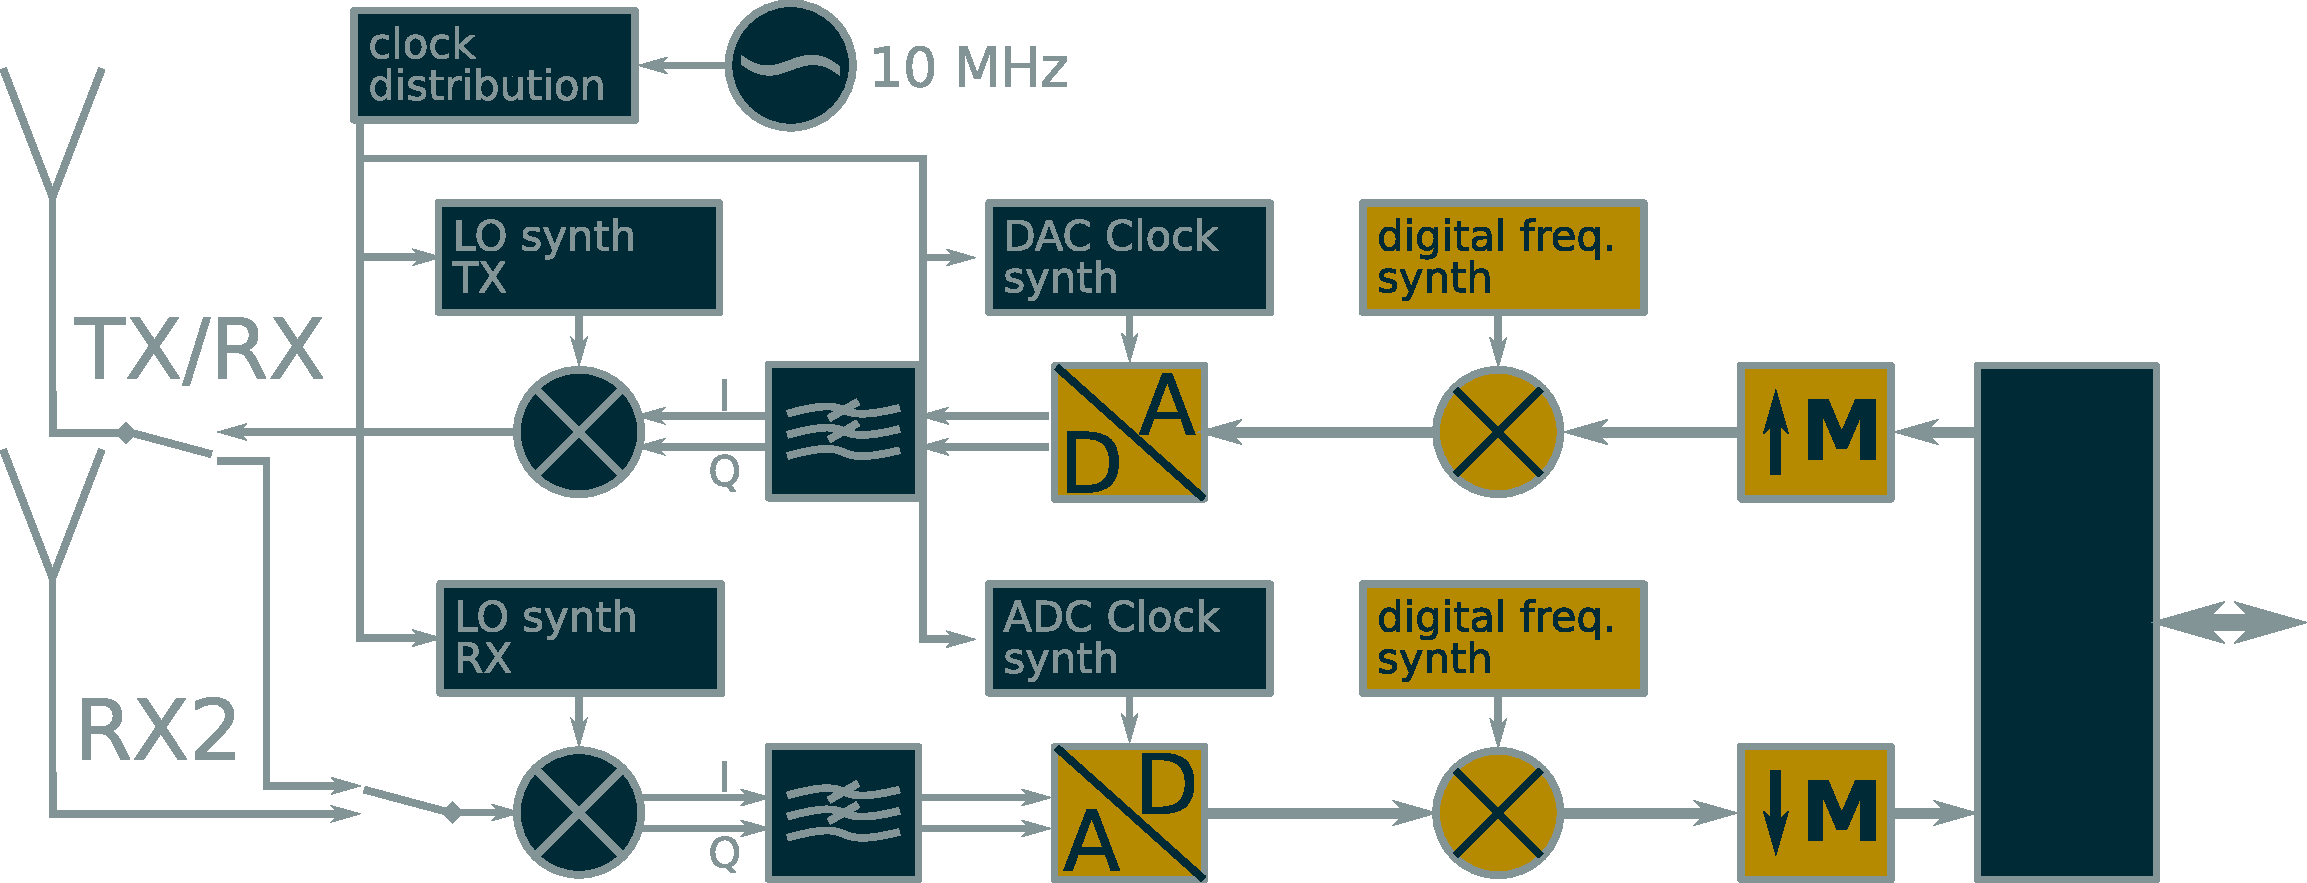
\includegraphics[width=\textwidth]{b200}}

\end{frame}

\begin{frame}{Looking at a complete system}

  FM Receiver in GNU Radio \bigskip

  {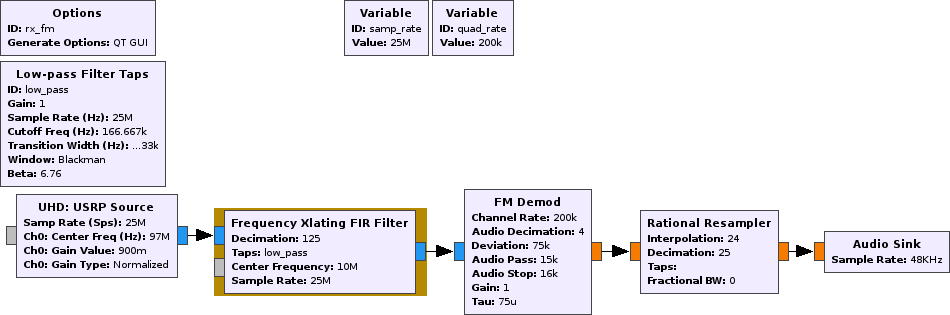
\includegraphics[width=\textwidth]{fg_xlating_fir}}


  Frequency Translating FIR filter

  \only<1>{\begin{itemize}
    \item shifts the desired frequency to 0 Hz
    \item then applies filter
    \item and decimates on the go
  \end{itemize}}
\end{frame}

\begin{frame}{Looking at a complete system}

  {\begin{itemize}
    \item 2045 tap monster of filter
    \item \ldots runs in real time on old laptop at up to 10 MS/s
    \item attenuation far above necessity
  \end{itemize}}
  {\includegraphics[width=\textwidth]{filterplot}}

\end{frame}
\begin{frame}{Looking at a complete system}

  FM Receiver in GNU Radio \bigskip

  {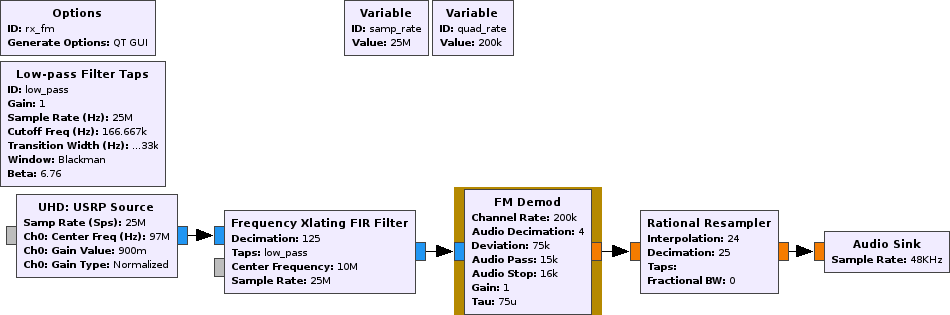
\includegraphics[width=\textwidth]{fg_fm_demod}}


  FM Demodulator

  {\begin{itemize}
    \item Calculates instantaneous frequency of signal
    \item integrates and scales the result
    \item and decimates to an audio-typical rate on the go
  \end{itemize}}

\end{frame}
\begin{frame}{Looking at a complete system}

  FM Receiver in GNU Radio \bigskip

  {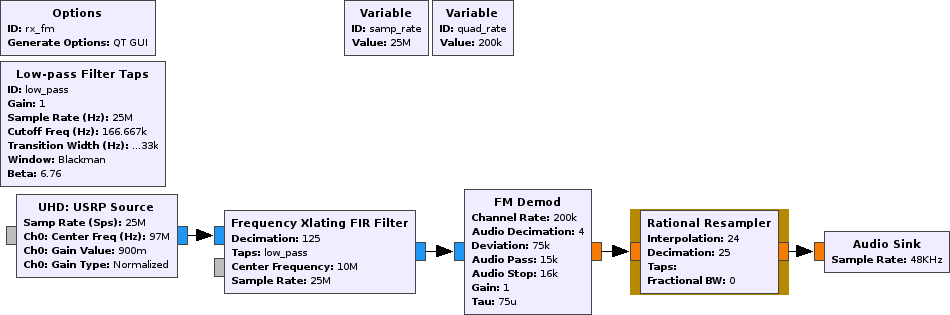
\includegraphics[width=\textwidth]{fg_resampler}}

  Rational Resampler

  {\begin{itemize}
    \item No sound card can do 50 kS/s, but they do 48 kS/s
      \begin{itemize}
        \item Interpolate to 48x input rate
        \item suppress spectral images
        \item filter and decimate by 50
      \end{itemize}
    \item In fact, there's tricks to do the downsampling, filtering and upsampling without going to 50x input rate
  \end{itemize}}



\end{frame}
\begin{frame}{Looking at a complete system}

  FM Receiver in GNU Radio \bigskip

  {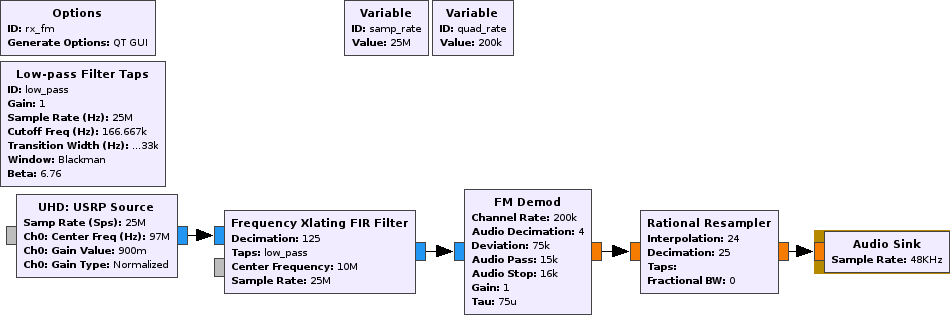
\includegraphics[width=\textwidth]{fg_audio_sink}}

  Audio Sink
  
  \begin{itemize}
    \item sends samples to the sound card, which Digital-to-Analog converts them
  \end{itemize}

\end{frame}

\section{Conclusion}
\begin{frame}{Conclusion}
  \begin{itemize}
    \item any signal is representable in digital form \ldots
    \item \ldots as long as it's band-limited
    \item Aliasing can lead to out-of-band overlaying wanted signal
    \begin{itemize}
      \item Anti-Alias Filtering necessary
      \item Aliasing can be used for good
    \end{itemize}
    \item DSP is a rich toolbox that allows construction of incredible filters at very low cost
    \item SDR hardware gives access to the raw digital signal -- great flexibility
    \item Toolboxes like GNU Radio make it very easy to build extremely capable SDR applications
  \end{itemize}
\end{frame}
\end{document}
